\chapter{Requirements}

\section{Functional requirements}

\subsection{Data Integration}

The Data Integration part of the platform needs to integrate several data sources to the Journal. Integration means that it must be able 
to detect the changes made to the data, and push events that can be either create event or update event or delete event.
In the following, we call a data entry a \textit{resource}. A resource is a keyed data defined by its id (for example \verb|/client/1| for a
resource of type client of id 1). Each type of resource has a defined set of fields (for example a client
will have a field name, address, ...).
\\

More specifically, the platform needs to integrate several data sources that expose REST APIs. Such APIs expose information
concerning business data such as new sales information, new financial information, new production information...
Each time that a resource is modified in one of these data sources, the platform should detect this change, apply some data cleaning and transformation, create an 
event from it and push it into the Journal.

The problem with most REST APIs is that they are not evented, i.e they are pulled-based and not pushed-based. 
One must sent an HTTP request to query new data each time they need to. There exists some techniques to stream data via HTTP 1.1 and the 
Chunked Transfer Encoding, but the REST APIs that the platform needs to integrate do not expose such stream interface. 
Thus, the architecture of this part needs to provide a way to perform incremental pull from data sources, and then transform
it in a push stream of events towards the Journal. Moreover, the platform needs to make sure to insert the events in the same
order that they happened in their data source.


\subsection{Journal and Stream Processing}

The Journal must provide a way for data producers to push one or several events that represent the creation, update or 
delete of a resource. Moreover, it must allow data consumers to subscribe to the stream of inserted events. Events must be
immutable and are stored in a sequence that respects the insertion order. The stream of events pushed to the data consumers
(stream processors) must be in the same order than the insertion order and with no event loss or duplication. Of course, the Journal must be persistent to
be able to recover its data after a shutdown or a crash.
\\

The Stream Processing part is the most complex part of the platform. This part should be a library that allows the user
to define a tree a stream processors (see Figure \ref{fig:tree}), where the root of the tree is the Journal. 

\begin{figure}[h]
  \begin{center} 
    \makebox[\textwidth]{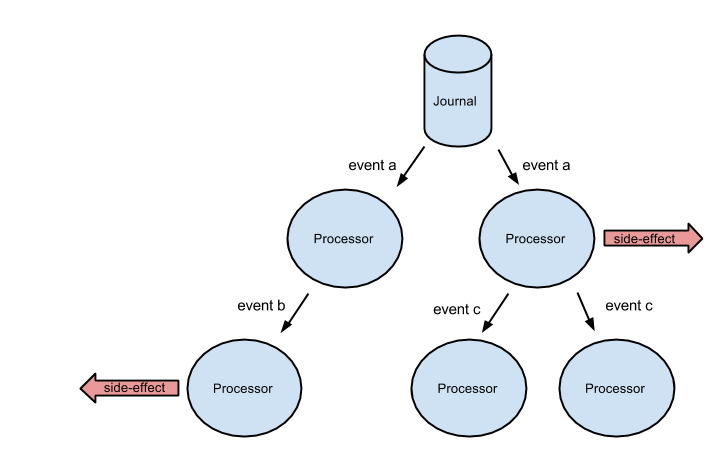
\includegraphics[width=1.0\textwidth]{img/tree.png}}
    \caption{A tree of stream processors}
    \label{fig:tree}
  \end{center}
\end{figure}

A stream processor receives events coming from its parent node. Upon the receive of an event, it can do one or several of these
actions (see Figure \ref{fig:streamprocessor}):
\begin{itemize}
  \item Creation of a sub-stream: the stream processor can transform a received event to a stream (several events), creating a sub-stream
  inside the global stream. The sub-stream must be inserted in-place in the stream: the whole sub-stream should be
  send in-order to the node's children before processing the next incoming event. For example, in Figure \ref{fig:substream},
  the processing of an input event 1 produces a sub-stream of out events 1-1, 1-2 and 1-3. Even if another input event 2
  arrives, it should not be processed before the whole sub-stream 1-1, 1-2 and 1-3 has been produced and sent to the processor's 
  children. This function is called \verb|process|.
  \item Side-effect with exactly-once semantics: The second action possible is to perform a side-effect upon each of the event
  of the sub-stream generated by the \verb|process| method. This side-effect can for example consist in updating a database representing
  a derived view on the data. This method, called \verb|performSideEffect|, must have an exactly-once semantic even in case of failures, so that the user
  can safely define non-idempotent side-effects.
\end{itemize}

\begin{figure}[h]
  \begin{center} 
    \makebox[\textwidth]{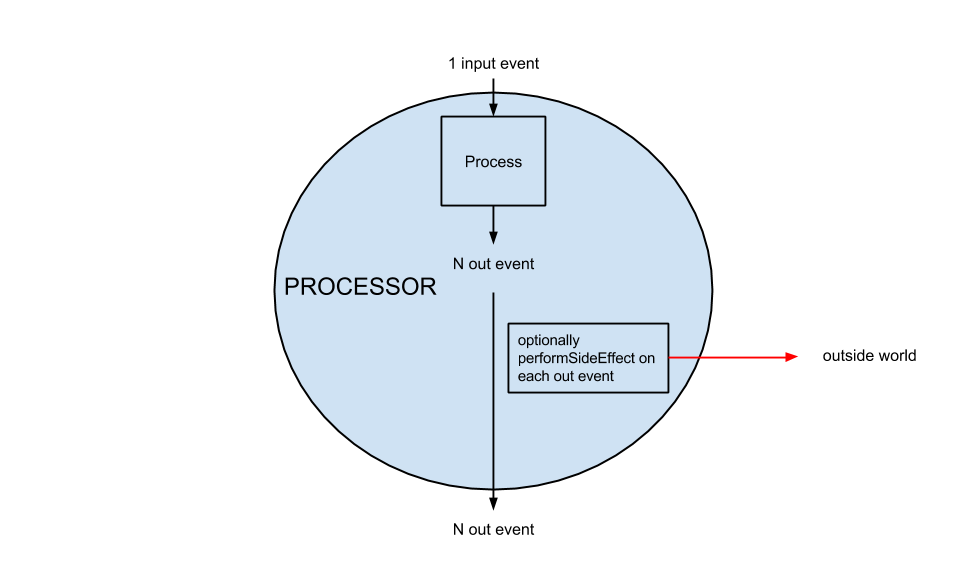
\includegraphics[width=1.0\textwidth]{img/stream_processor.png}}
    \caption{A stream processor}
    \label{fig:streamprocessor}
  \end{center}
\end{figure}

\begin{figure}[h]
  \begin{center} 
    \makebox[\textwidth]{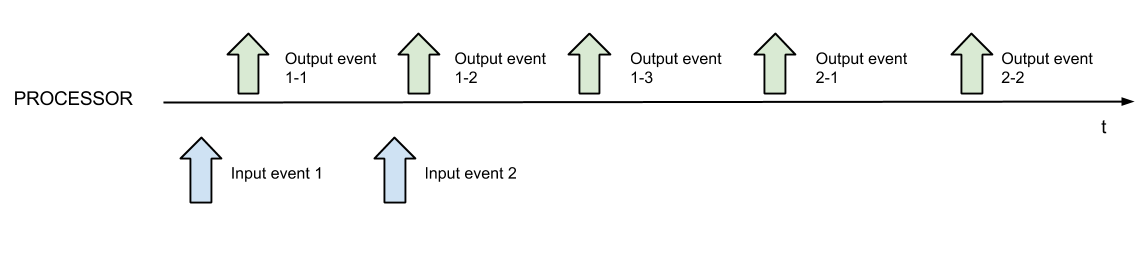
\includegraphics[width=1.0\textwidth]{img/substream.png}}
    \caption{In-order insertion of a sub-stream in a stream}
    \label{fig:substream}
  \end{center}
\end{figure}

Another important functional requirement for processors is that the \verb|process| and \verb|performSideEffect| methods can ensure the
sequentiality of asynchronous non-blocking operations (for example, a side-effect or a processing can be done via an asynchronous call to a 
database, but despite the asynchronous nature of the call the processor must wait that the asynchronous call has returned
before processing the next event). Even sub-stream production can be asynchronous, meaning that the production of a sub-stream
can be a composition of asynchronous operations (like pulling from a database with an asynchronous non-blocking driver).

\section{Non-functional requirements}

\subsection{Data Integration}

The Data Integration part must be able to scale up easily. Scale up means that the puller should automatically make the best
use possible of all cores available on a machine in order to parallelize the various pulls. The different parts of the puller 
should also be easily distributable in case of the load if too big for one machine to handle. 

The puller should also be fault-tolerant, meaning that a failure and restart of the system should ensure that no event
is duplicated or lost.

Moreover, the nature of the puller implies that it will spend the majority of its time doing IO to query different data sources.
Those IOs can have various durations depending on the size of the data to pull, the latency and bandwidth of the data sources, etc.
We want to optimize the use of resource (CPU, RAM) despite the fact that the platform is very IO-oriented. Chapter \ref{chap:study} will show how asynchronous non-blocking IO meets these expectations.

Another non-functional requirement is to have clean and composable code source despite its asynchronous nature. Asynchronous
code can indeed lead to maintenance nightmare if the wrong abstractions are used. Chapter \ref{chap:study} will
show that the use of functional programming solves these problems.

\subsection{Journal and Stream Processing}

The Journal and Stream Processing part requires complex non-functional requirements in order to optimize resource consumption and maximize performance.

A common problem with stream processing is to manage the flow rate. A producer can indeed produce events at a rate superior to
the processing rate of a consumer. This problem is even more important when there is
a tree-like structure of stream processors instead of a linear structure. Indeed, the platform should handle the fact that even if sibling processors in the tree
have different processing speeds, they do not block each other based on the slowest sibling. In other words, sibling processors should be
totally decoupled so that when a new event is sent from a parent to its children, the parent does not have to wait that its slowest
children has finished to process the event in order to send the next event to them. This problem should be handled while minimizing
RAM consumption.

Another requirement is no message loss or duplication even in case of a temporary failure of a processor. This means that a processor
that had a transient failure must be able to \textit{replay} the stream from where it was before its crash.

Stream processors should also be easily distributable in order to deal with event flows that are too big
for one machine to handle.


